\subsection{Arcos y homotopias}
Para la construccion de nuestra invariante, debemos de familiarizarnos
con los arcos y las deformaciones continuas entre ellos llamadas
\emph{homotopias}.

\begin{definicion}[Arco]
  Un arco en el espacio \(X\) es una funcion continua \(f : I \to X \)
  donde \(I = [0,1]\)
\end{definicion}
La definicion tradicional es ligeramente mas general cambiando que \(I\)
sea un subconjunto convexo acotado de un espacio unidimensional, pero
siempre podemos recuperar esta definicion rescalando la distancia.

\begin{definicion}[Homotopia]
  Dados dos arcos \(f,g : I \to X\), diremos que \(f\) es homotopico a
  \(g\) si existe una funcion continua \(F : I \times I \to X \) tal que
  \[ \begin{matrix}
      F (x, 0) = f(x) & F (x, 1) = g(x)
     \end{matrix}
  \]
  Donde \(F\) sera llamada una homotopia entre \(f\) y \(g\). La
  existencia de dicha relacion entre dos funciones sera denotada por \(f
  \homRelAlt g\).
\end{definicion}
\begin{figure}[h]
  \centering
  \includegraphics[scale=0.5]{./imagenes/homotopia.png}
  \caption{caracterizacion homotopia}
  \label{fig:homotopia-entre-funciones}
\end{figure}
Podemos pensar en el segundo argumento de una homotopia como el grado de
deformación entre dos funciones.
Si tratamos con arcos \(f,g : I \to X\) que posean los mismos puntos
iniciales y finales, es decir \(f(0) = g(0) = x_0, \; f(1) = g(1) =
x_1 \) podemos definir una relacion homotopica ligeramente mas fuerte.

\begin{definicion}[Arco homotopia]
  \(f,g : I \to X\) son \emph{arco homotopicas} entre sí, si tienen los mismos
  puntos inicial y final \(x_0, x_1\) respectivamente y existe una homotopia entre
  ellos tal que cumpla
  \[
    \begin{matrix}
      F(s,0) = f(s) & F(s,1) = g(s) \\
      F(0,t) = x_0  & F(1,t) = x_1
    \end{matrix}
  \]
  La existencia de esta relacion entre dos funciones sera denotada por
  \(f \simeq g\).
\end{definicion}
% todo(slack) hacer algun dibujo de las homotopias entre las curvas
Una vez definida estas relaciones, una pregunta natural es si estas definen
una relacion de equivalencia, ya que nos gustaria identificar clases de
curvas como elementos de alguna teoria algebraica. La respuesta es
afirmativa para ambas relaciones (el punto de inicio y final no juegan
papel), se mostrara para las homotopias.

\begin{teorema}
  \(\homRelAlt\) es una relacion de equivalencia
\end{teorema}
\begin{proof}
  Hemos de probar que esta relacion cumple la reflexividad, simetria y
  transitividad. Sean \(f,g,h : I \to X\) tres arcos arbitrarios.
  \begin{itemize}
  \item La reflexividad es directa pues la funcion \(F(x,t) = f(x)\) es
    una deformacion continua de \(f\) a \(f\), por tanto \(f \homRelAlt
    f\).

  \item La simetria se obtiene de invertir el grado de deformacion de la
    homotopia original. Formalmente, dado \(f \stackrel{.}{\simeq} g\)
    tenemos una homotopia entre estas \((x,t) \mapsto F(x,t)\). A partir
    de aqui podemos definir
    \begin{equation}
      \label{eq:homotopy-simetry}
      (x,t) \mapsto \hat{F}(x,t) := F(x,1-t)
    \end{equation}
    con \(\hat{F}\) una homotopia entre \(g\) y \(f\). Por tanto \(g
    \stackrel{.}{\simeq} f\).


  \item La transitividad se obtiene a partir de de dividir \(I\) en dos
    intervalos donde se deformen individualmente cada homotopia al doble
    del grado. Formalmente dado \(f \stackrel{.}{\simeq} g\) y \(g
    \stackrel{.}{\simeq} h\) representadas por las homotopias \(F\) y
    \(G\) respectivamente, se define
    \[ FG(x,t) = \begin{cases}
        F(x,2t) & t \in [0,\frac{1}{2}] \\
        G(x,2t - 1) & t \in [ \frac{1}{2} , 1]
      \end{cases}
    \]
    Esta es una deformacion continua claramente en \((x,t) \in I \times
    [0, \frac{1}{2}) \cup I \times (\frac{1}{2}, 1]\). La continuidad en
    \(I \times \{\frac{1}{2}\}\) proviene de la consistencia en dicho
    punto de ambas homotopias
    \[ F(x,2 \cdot \frac{1}{2}) = g(x) = G(x, 2 \cdot \frac{1}{2} - 1)\]
    lo que nos permite utilizar el lema del pegamiento para obtener la
    continuidad de \(FG\). Obteniendo asi \(f \stackrel{.}{\simeq} h\).
  \end{itemize}
\end{proof}

En analisis real, es comun trabajar con conjuntos convexos, en arcos
sobre estos, veremos una homotopia usual repetidamente que es llamada
homotopia de linea recta.
\begin{definicion}\label{def:homotopia-linea}
  Sean \(f,g : I \to X\) dos arcos arbitrarios. Si \(f(I),g(I) \subset
  \mathcal C\), subconjunto convexo de \(X\), entonces
  \[ (x,t) \mapsto F(x,t) = (1-t) \cdot f(x) + t \cdot g(x) \]
  Es una homotopia entre \(f\) y \(g\), la cual es continua en virtud de
  ser combinacion lineal de funciones continuas.
\end{definicion}

Con estas definiciones ya podemos empezar a hablar de \([f]\) clases
de equivalencia de funciones bajo una relacion homotopica
\[ [f] = \{ g : I \to X \mid f \stackrel{.}{\simeq} g \} \]
Notar que la construccion es valida para las dos relaciones aunque por
nuestra meta de construir el grupo fundamental nos interesa
principalmente la relacion arco homotopica, por razones a estudiar mas
adelante.
